\documentclass[a4paper, 10.5pt, notitlepage]{article}
\usepackage[margin=3cm]{geometry}
\usepackage{listings}
\usepackage[parfill]{parskip}
\setlength{\parskip}{\baselineskip}%
\setlength{\parindent}{0pt}%
\usepackage{amsmath}
\usepackage{amssymb}
\usepackage{graphicx}
\usepackage[justification=centering]{caption}
\usepackage{epstopdf}
\usepackage[usenames, dvipsnames]{color}
\usepackage{chngcntr}
\usepackage{titling}
%\counterwithout{footnote}{chapter}
\usepackage{float}
%\renewcommand\theContinuedFloat{\alph{ContinuedFloat}}
\newcommand\tab[1][0.05cm]{\hspace*{#1}}

\title{Numerical Assignment}
\author{Mariana Clare}
\date{\today}

\begin{document}
	
\maketitle
\thispagestyle{empty}
\section{Introduction}
This report seeks to solve the one-dimensional lineriased shallow water equations using four different numerical methods: Co-located Explicit, Co-located Implicit, Staggered Explicit and Staggered Implicit. It also compares the error between these methods and the analytic solutions for given initial conditions, as well as testing their stability and computational cost and evaluating how physically realistic they are.

The shallow water equations are
\begin{equation}\label{momentumsw}
\frac{\partial \mathbf{u}}{\partial t} + \mathbf{u}\cdot\nabla\mathbf{u} = - 2\Omega \times\mathbf{u} - g\nabla (h + h_{0})
\end{equation}
\begin{equation}\label{masssw}
\frac{\partial h}{\partial t} + \mathbf{u}\cdot\nabla h = - h \nabla \cdot \mathbf{u}
\end{equation}
where $\mathbf{u}$ is the velocity of the flow, $\Omega$ the angular velocity of the rotating frame of reference, $g$ the gravitational acceleration constant, $h$ the depth of the fluid and $h_{0}$ represents the underlying shape the fluid is flowing over (as defined in \cite{MPE textbook}). Equation (\ref{momentumsw}) represents the conservation of momentum and equation (\ref{masssw}) represents the conservation of mass.

Following \cite{MPE textbook}, we consider the one-dimensional form of these equations and linearise them about the state $u = 0$ and $h = H$, \textit{ie.}
\begin{eqnarray}
\mathbf{u} =  & \mathbf{\hat{u}}
 \\   \nonumber
h = &  H + \hat{h} .
\end{eqnarray}
where $H$ is the average fluid depth. We further assume that $h_{0}$ is constant and the frame is not rotating. Dropping the $\hat{}$ notation this gives
\begin{equation}\label{linearisedsw1}
\frac{\partial u}{\partial t} = - g \frac{\partial h}{\partial x}
\end{equation}
\begin{equation}\label{linearisedsw2}
\frac{\partial h}{\partial t} = - H \frac{\partial u}{\partial x}.
\end{equation}
\textit{N.B.} Throughout this report we assume for simplicity that $u$ and $h$ have periodic boundary conditions.

\section{Numerical Methods}\label{numericalmethodssection}

\subsection {Co-located Explicit}
The first numerical method we use to solve (\ref{linearisedsw1}) and (\ref{linearisedsw2}) is a simple co-located forward-backward in time and centred in space explicit scheme. As in \cite{MPE textbook}, we consider the scheme to be forward in time for $u$ and backward in time for $h$. Co-located (sometimes referred to as A-grid) means we define the velocity and the height at the same location on the meshgrid.

This scheme can be written as 
\begin{equation} \label{FTCSAgrid}
\frac{u_{j}^{(n+1)} - u_{j}^{(n)}}{\Delta t} = -g \frac{h_{j+1}^{(n)} - h_{j-1}^{(n)}}{2\Delta x}
\end{equation}
\begin{equation}\label{BTCSAgrid}
\frac{h_{j}^{(n+1)} - h_{j}^{(n)}}{\Delta t} = -H \frac{u_{j+1}^{(n+1)} - u_{j-1}^{(n+1)}}{2\Delta x}
\end{equation}
where $h_{j}^{(n)} = h(x_{j}, t^{(n)})$, $u_{j}^{(n)} = h(u_{j}, t^{(n)})$, $x_{j} = j\Delta x$ and $t^{(n)} = n\Delta t$. 

We can determine the order of accuracy of this scheme, by using a Taylor series expansion. From \cite{MPE textbook}, we know that both the forward in time and centred in space and the backward in time and centred in space schemes are first order accurate in time and second order accurate in space. Therefore the co-located explicit scheme is also first order accurate in time and second order accurate in space.

We use a Von-neumann stability analysis to determine when this scheme is stable. As in \cite{MPE textbook}, we assume that $u$ and $h$ have wave-like solutions with an amplification factor $A$ and wavenumber $k$ for constant $\mathbb{U}$ and $\mathbb{H}$:
\begin{equation} \label{wavelikeu}
u  =  \mathbb{U}  A^{n} e^{ikj\Delta x}
\end{equation}
\begin{equation} \label{wavelikeh}
h  =  \mathbb{H} A^{n} e^{ikj\Delta x}
\end{equation}

Furthermore if we define the Courant number 
\begin{equation}\label{Courantnumber}
c = \frac{\sqrt{gH}\Delta t}{\Delta x}
\end{equation}
then substituting these solutions into (\ref{FTCSAgrid}) and (\ref{BTCSAgrid}) gives
\begin{equation}
A = 1 - \frac{c^{2}}{2} \sin^{2}(k\Delta x) \pm \frac{ic}{2}\sin(k\Delta x)\sqrt{4 - c^{2}\sin^{2}k\Delta x}.
\end{equation} 
 
Hence and as stated in \cite{MPE textbook}, when $\lvert c \rvert \leq 2$, $\lvert A \rvert^{2} = 1$ the scheme is stable, and when $\lvert c \rvert > 2$, it is unstable (\textit{ie.} $\vert A \rvert > 1$ for some $k\Delta x$).
 
We can also find the dispersion relation, because the frequency of the numerical method is 
\begin{equation} \label{frequency}
\omega = \pm \frac{1}{\Delta t} \arctan\bigg(\frac{Im(A)}{Re(A)}\bigg).
\end{equation}
Hence and again as stated in \cite{MPE textbook}, 
\begin{equation}
\omega_{n}\Delta x = \pm \frac{2}{c} \sin^{-1} \bigg(\frac{c}{2}\sin(k\Delta x)\bigg),
\end{equation}
assuming $\sqrt{gH} = 1$. The positive branch of this dispersion relation is plotted in Figure \ref{dispersionfigure} and compared with that of the analytic solution. This shows that the two solutions do not propagate at the same rate. The numerical solution disperses too slowly and in fact grid-scale waves (where $k\Delta x = \pi$) are stationary.

Note that the dispersion relation of the analytic solution $\omega = k\sqrt{gH}$ is found by substituting the wave-like solutions (\ref{wavelikeu}) and (\ref{wavelikeh}) into (\ref{linearisedsw1}) and (\ref{linearisedsw2}). 

\subsection{Co-located Implicit}
We would prefer to have a method that is stable for all Courant numbers. A good method we can use is the implicit method on a co-located grid. As in \cite{MPE textbook}, we consider the co-located scheme which is backward in time and centered in space for both $u$ and $h$:
\begin{equation} \label{FTimplicitAgrid1}
\frac{u_{j}^{(n+1)} - u_{j}^{(n)}}{\Delta t} = -g \frac{h_{j+1}^{(n+1)} - h_{j-1}^{(n+1)}}{2\Delta x}
\end{equation}
\begin{equation}\label{FTimplicitAgrid2}
\frac{h_{j}^{(n+1)} - h_{j}^{(n)}}{\Delta t} = -H \frac{u_{j+1}^{(n+1)} - u_{j-1}^{(n+1)}}{2\Delta x}.
\end{equation}

To find the values of $h_{j}^{n}$ and $u_{j}^{n}$ at the following time iteration for all $j$, we consider the matrix, where $c$ is the Courant number as before:

\[
B = \left (
\begin{array}{ccc}
\begin{array}{ccccc}
1 + \frac{c^{2}}{2} & 0 & -\frac{c^{2}}{4} & 0 & 0\\
0& 1 + \frac{c^{2}}{2} & 0 & -\frac{c^{2}}{4} & 0\\
-\frac{c^{2}}{4} & 0& 1 + \frac{c^{2}}{2} & 0 & -\frac{c^{2}}{4}\\
\vdots & & \vdots & & \vdots\\
- \frac{c^{2}}{4} & 0 & 0 & 0 & 0\\
0 & - \frac{c^{2}}{4} & 0 & 0 & 0\\
\end{array}
\begin{array}{c}
\vdots\\ 
\ddots\\
\vdots
\end{array}
\begin{array}{ccccc}
0 & 0 & 0 & - \frac{c^{2}}{4} & 0\\
0 & 0 & 0 & 0 & - \frac{c^{2}}{4}\\
\vdots & & \vdots & & \vdots\\
-\frac{c^{2}}{4}& 0 & 1 + \frac{c^{2}}{2} & 0 & -\frac{c^{2}}{4} \\
0 & -\frac{c^{2}}{4} & 0 & 1 + \frac{c^{2}}{2} & 0\\
0 & 0 & -\frac{c^{2}}{4}& 0 & 1 + \frac{c^{2}}{2}
\end{array}
\end{array}
\right )
\]

We can write (\ref{FTimplicitAgrid1}) and (\ref{FTimplicitAgrid2}) as the matrix equation $B \mathbf{x} = \mathbf{b}$ where $\forall j \in [0, N-1]$
\begin{eqnarray}
x_{j} & = & u_{j}^{(n+1)}\\
b_{j} & = & u_{j}^{(n)} - \frac{c}{2}\sqrt{\frac{g}{H}}\bigg(h_{j+1}^{(n)} - h_{j-1}^{(n)}\bigg) 
\end{eqnarray}
if solving for $u$ and 
\begin{eqnarray}
x_{j} & = & h_{j}^{(n+1)}\\
b_{j} & = & h_{j}^{(n)} - \frac{c}{2}\sqrt{\frac{H}{g}}\bigg(u_{j+1}^{(n)} - u_{j-1}^{(n)}\bigg)
\end{eqnarray}
if solving for $h$.

Furthermore, as we are assuming periodic boundary conditions, $u_{0}^{(n)} = u_{N}^{(n)}$ and $h_{0}^{(n)} = h_{N}^{(n)}$ where $N\Delta x$ is the maximum value of $x$ in the $x$-domain. Hence the matrix $B$ has dimension $N \times N$ and we consider the first row to be $j = 0$. 

We can determine the order of accuracy of this scheme, as before, by using a Taylor series expansion.  From \cite{MPE textbook}, we know that both the backward in time and centred in space scheme is first order accurate in time and second order accurate in space. Therefore the staggered explicit scheme is also first order accurate in time and second order accurate in space.

Again we use Von-Neumann stability analysis to find where this scheme is stable and assume $u$ and $h$ have wave-like solutions (\ref{wavelikeu}) and (\ref{wavelikeh}). Substituting these solutions into (\ref{FTimplicitAgrid1}) and (\ref{FTimplicitAgrid2}) we find
\begin{equation}
A = \frac{1 \pm i c\sin(k\Delta x)}{1 + c^{2}\sin^{2}(k\Delta x)}
\end{equation}
Therefore $\lvert A \rvert ^{2} < 1$ and the scheme is uncondtionally stable (\textit{ie.} stable for all Courant numbers). 

Using (\ref{frequency}) we can find the dispersion relation
\begin{equation}
\omega_{n} \Delta x = \pm\frac{\Delta x}{\Delta t} \arctan(c\sin(k\Delta x)) = \frac{1}{c}  \arctan(c\sin(k\Delta x))
\end{equation}
assuming $\sqrt{gH} = 1$. The positive branch of this dispersion relation is again plotted in Figure \ref{dispersionfigure}. As with the explicit scheme, the numerical solution is dispersive and propagates too slowly and again grid-scale waves (where $k\Delta x = \pi$) are stationary. 

\subsection{Staggered Explicit}
Next we seek a scheme which propagates at a speed more similar to that of the analytic solution. Following \cite{MPE textbook}, we use a staggered grid (sometimes known as a C-grid) instead of a co-located grid. For a staggered grid, we shift $u$ so that it is defined at $x_{j} + \frac{\Delta x}{2}$ and $h$ remains defined at $x_{j}$ (where $x_{j} = j \Delta x$) \textit{ie.} $u$ and $h$ are defined alternately in space.

As in \cite{MPE textbook}, we take again the forward-backward in time and centred in space scheme where the scheme is forward in $u$ and backward in $h$, but now we use a staggered grid. This gives us the following scheme:

\begin{equation}\label{FTCSCgrid}
\frac{u_{j+ \frac{1}{2}}^{(n+1)} - u_{j + \frac{1}{2}}^{(n)}}{\Delta t} = -g \frac{h_{j+1}^{(n)} - h_{j}^{(n)}}{\Delta x}
\end{equation}

\begin{equation}\label{BTCSCgrid}
\frac{h_{j}^{(n+1)} - h_{j}^{(n)}}{\Delta t} = -H \frac{u_{j+\frac{1}{2}}^{(n+1)} - u_{j-\frac{1}{2}}^{(n+1)}}{\Delta x}
\end{equation}


We can determine the order of accuracy of this scheme on a staggered grid by using the following Taylor series expansion 
\begin{equation}
h_{j + 1}^{(n)} = h_{j}^{(n)} + \Delta x  \frac{\partial h_{j}^{(n)}}{\partial x} + \frac{\Delta x^{2}}{2}\frac{\partial^{2} h_{j}^{(n)}}{\partial x^{2}} + \frac{\Delta x^{3}}{6}\frac{\partial^{3} h_{j}^{(n)}}{\partial x^{3}} + O(\Delta x^{4})
\end{equation}
\begin{equation} \label{uj+1/2n}
u_{j \pm \frac{1}{2}}^{(n)} = u_{j}^{(n)} \pm \frac{\Delta x}{2}\frac{\partial u_{j}^{(n)}}{\partial x} + \frac{\Delta x^{2}}{8}\frac{\partial^{2}u_{j}^{n}}{\partial x^{2}} + O(\Delta x^{3})
\end{equation}
\begin{equation} \label{uj+1/2n+1}
u_{j \pm \frac{1}{2}}^{(n + 1)} = u_{j}^{(n)} \pm \frac{\Delta x}{2}\frac{\partial u_{j}^{(n)}}{\partial x} + \Delta t \frac{\partial u_{j}^{(n)}}{\partial t} + \frac{\Delta x^{2}}{8}\frac{\partial^{2}u_{j}^{n}}{\partial x^{2}} \pm \frac{\Delta t \Delta x}{2}\frac{\partial^{2} u_{j}^{(n)}}{\partial x \partial t} + \frac{\Delta t^{2}}{2} \frac{\partial ^{2} u_{j}^{(n)}}{\partial t ^{2}} + O(\Delta x^{3}, \Delta t^{3})
\end{equation}

Substituting these into (\ref{FTCSCgrid}), we find that 
\begin{equation}
\frac{\partial u_{j}^{(n)}}{\partial t} + O(\Delta t) =  -g \frac{\partial h_{j}^{(n)}}{\partial x} + O(\Delta x^{2})
\end{equation} 
and therefore the scheme is first order accurate in time and second order accurate in space. (Note the same order of accuracy is obtained by performing the same analysis with equation (\ref{BTCSCgrid})).

Again we use Von-Neumann stability analysis to find where this scheme is stable, and assume that $u$ and $h$ have wave-like solutions (\ref{wavelikeu}) and (\ref{wavelikeh}). Substituting these solutions into (\ref{FTCSCgrid}) and (\ref{BTCSCgrid}), we find
\begin{equation}
A = 1 - 2c^{2}\sin^{2}\bigg(\frac{k\Delta x}{2}\bigg) \pm 2ic\sin\bigg(\frac{k\Delta x}{2}\bigg) \sqrt{1 - c^{2}\sin^{2}\bigg(\frac{k\Delta x}{2}\bigg)}
\end{equation}
Therefore if $\lvert c \rvert \leq 1$ this scheme is stable and if $\lvert c \rvert > 1$ it is unstable  (\textit{ie.} $\vert A \rvert > 1$ for some $k\Delta x$).

Using (\ref{frequency}) we can find the dispersion relation
\begin{equation}
	\omega_{n} \Delta x = \pm\frac{2\Delta x}{\Delta t} \arcsin\bigg(c\sin\bigg(\frac{k\Delta x}{2}\bigg)\bigg) = \frac{2}{c} \arcsin\bigg(c\sin\bigg(\frac{k\Delta x}{2}\bigg)\bigg) 
\end{equation}
assuming $\sqrt{gH} = 1$. The positive branch of this dispersion relation is again plotted in Figure \ref{dispersionfigure}. Although this solution is still dispersive and still propagates too slowly, we can see from the Figure that $\omega$ of this numerical scheme approximates much more closely $\omega$ of the analytic solution. Importantly as $k\Delta x$ increases, $\omega$ is always increasing. Furthermore, we no longer have a value for $k\Delta x$ for which the wave is stationary (as the maximum values of $k\Delta x$ is $\pi$).

\subsection{Staggered Implicit}
The staggered explicit method has again the problem that the solution is unstable for some Courant numbers. Therefore the final numerical method we look at is the implicit scheme on a staggered grid, as outlined in \cite{implicit}. The method suggested in \cite{implicit} is the theta-method:
\begin{equation}
\frac{u_{j + \frac{1}{2}}^{(n + 1)} - u_{j + \frac{1}{2}}^{(n)}}{\Delta t} = -\frac{g}{\Delta x} \bigg(\theta (h_{j + 1}^{(n+ 1)} - h_{j}^{(n+ 1)}) + (1 - \theta) (h_{j + 1}^{(n)} - h_{j}^{(n)})\bigg),
\end{equation}
\begin{equation}
\frac{h_{j}^{(n + 1)} - h_{j}^{(n)}}{\Delta t} = -\frac{H}{\Delta x} \bigg(\theta (u_{j + \frac{1}{2}}^{(n+ 1)} - u_{j - \frac{1}{2}}^{(n+ 1)}) + (1 - \theta) (u_{j + \frac{1}{2}}^{(n)} - u_{j - \frac{1}{2}}^{(n)})\bigg).
\end{equation}

In \cite{implicit} it is shown that if we take $\theta = \frac{1}{2}$ the scheme is second order accurate. Therefore, we take $\theta = \frac{1}{2}$ and use the Crank-Nicholson method centred in space on a staggered grid to get
\begin{equation}\label{semiimplicit1}
\frac{u_{j + \frac{1}{2}}^{(n + 1)} - u_{j + \frac{1}{2}}^{(n)}}{\Delta t} = -\frac{g}{2\Delta x} \bigg(h_{j + 1}^{(n+ 1)} - h_{j}^{(n+ 1)} + h_{j + 1}^{(n)} - h_{j}^{(n)}\bigg)
\end{equation}
\begin{equation}\label{semiimplicit2}
\frac{h_{j}^{(n + 1)} - h_{j}^{(n)}}{\Delta t} = -\frac{H}{2\Delta x} \bigg(u_{j + \frac{1}{2}}^{(n+ 1)} - u_{j - \frac{1}{2}}^{(n+ 1)} + u_{j + \frac{1}{2}}^{(n)} - u_{j - \frac{1}{2}}^{(n)}\bigg)
\end{equation}

In order to find the values of $h_{j}^{n}$ and $u_{j}^{n}$ at the following time iteration for all $j$, we consider the matrix where $c$ is the Courant number as before:

\[
B = \left (
\begin{array}{ccc}
\begin{array}{ccc}
1 + \frac{c^{2}}{2} & -\frac{c^{2}}{4} & 0\\
-\frac{c^{2}}{4}& 1 + \frac{c^{2}}{2} & -\frac{c^{2}}{4} \\
\vdots & \vdots & \vdots\\
0 & 0  & 0 \\
- \frac{c^{2}}{4}  & 0  & 0 
\end{array}
\begin{array}{c}
\vdots\\ 
\ddots\\
\vdots
\end{array}
\begin{array}{ccc}
0  & 0  &  - \frac{c^{2}}{4}\\
0  & 0& 0\\
\vdots & \vdots & \vdots\\
-\frac{c^{2}}{4}& 1 + \frac{c^{2}}{2} & -\frac{c^{2}}{4} \\
0 & -\frac{c^{2}}{4} & 1 + \frac{c^{2}}{2}
\end{array}
\end{array}
\right )
\]

We can write (\ref{semiimplicit1}) and (\ref{semiimplicit2}) as the matrix equation $B \mathbf{x} = \mathbf{b}$ where $ \forall j \in [0, N-1]$
\begin{eqnarray}
x_{j} &= & u_{j}^{(n+1)}\\
b_{j} &= & -c\sqrt\frac{g}{H}\bigg(h_{j + 1}^{(n)} - h_{j}^{n}\bigg) + \frac{c^{2}}{4} u_{j + \frac{3}{2}}^{(n)} + \bigg(1 - \frac{c^{2}}{2}\bigg)u_{j + \frac{1}{2}}^{(n)} + \frac{c^{2}}{4} u_{j - \frac{1}{2}}^{(n)}
\end{eqnarray}
if solving for $u$ and
\begin{eqnarray}
x_{j} & =& h_{j+ \frac{1}{2}}^{(n+1)} \\
b_{j} &= &-c\sqrt\frac{H}{g}\bigg(u_{j + \frac{1}{2}}^{(n)} - u_{j - \frac{1}{2}}^{n}\bigg) + \frac{c^{2}}{4} h_{j + 1}^{(n)} + \bigg(1 - \frac{c^{2}}{2}\bigg)h_{j}^{(n)} + \frac{c^{2}}{4} h_{j - 1}^{(n)}
\end{eqnarray}
if solving for $h$.

Furthermore, as we are assuming periodic boundary conditions, $u_{\frac{1}{2}}^{(n)} = u_{N + \frac{1}{2}}^{(n)}$ and $h_{0}^{(n)} = h_{N}^{(n)}$ where $N\Delta x$ is the maximum value of $x$ in the $x$-domain. Hence, the matrix $B$ has dimension $N \times N$ and we consider the first row to be $j = 0$.

From \cite{implicit} the scheme is second order accurate in time and second order accurate in space, which is more accurate than any of the other schemes we have looked at so far.

As before we use Von-Neumann stability analysis to find where the scheme is stable, and assume that $u$ and $h$ have wave-like solutions (\ref{wavelikeu}) and (\ref{wavelikeh}). Substituting these solutions into (\ref{semiimplicit1}) and (\ref{semiimplicit2}) we find
\begin{equation}
A = \frac{1 - c^{2}\sin^{2}(\frac{k\Delta x}{2}) \pm 2ic\sin(\frac{k\Delta x}{2})}{1 + c^{2}\sin^{2}(\frac{k\Delta x}{2})}
\end{equation}
and $\lvert A \rvert^{2} = 1$. Therefore the scheme is unconditionally stable (\textit{ie.} stable for all Courant numbers) $\forall k$.

Using (\ref{frequency}), we can find the dispersion relation
\begin{equation}
\omega_{n} \Delta x = \pm\frac{\Delta x}{\Delta t} \arctan\bigg(\frac{2 c \sin(\frac{k\Delta x}{2})}{1 - c^{2} \sin^{2}(\frac{k\Delta x}{2})}\bigg) = \pm\frac{1}{c} \arctan\bigg(\frac{2 c \sin(\frac{k\Delta x}{2})}{1 - c^{2} \sin^{2}(\frac{k\Delta x}{2})}\bigg)
\end{equation}
assuming $\sqrt{gH} = 1$. The positive branch of this dispersion relation is also plotted in Figure \ref{dispersionfigure}. 

As with the previous staggered grid scheme, this solution is dispersive. However, as with the explicit staggered grid scheme, as $k\Delta x$ increases $\omega$ increases and $\omega$ approximates much more closely $\omega$ of the analytic solution than either of the co-located schemes. Furthermore there are no values of $k\Delta x$ for which the wave is stationary. The dispersion relation for the implicit staggered scheme diverges more from the analytic solution than the explicit staggered scheme but the difference is very small. 

\begin{figure}[H]
	\begin{center}

	\centering
	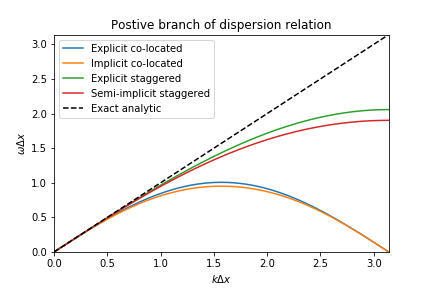
\includegraphics[width=0.6\textwidth]{dispersion_relations.png}
	\caption{Positive branch of dispersion relation $\omega$ for analytic solution and numerical methods. Note that as in \cite{MPE textbook}, we have used $c=0.4$ and $\sqrt{gH} = 1$.} \label{dispersionfigure}

	\end{center}
\end{figure}

\section{Results}\label{resultssection}
We now conduct a series of tests on a variety of initial conditions to examine the numerical methods outlined in the above section. Note that for all the follwing results we define:
\begin{eqnarray}
H & = & 1\\
g & = & 1
\end{eqnarray}
where $H$ is the average fluid depth and $g$ is the gravitational acceleration constant.

\renewcommand\theContinuedFloat{\alph{ContinuedFloat}}
\begin{figure}[H]
	\begin{minipage}{.5\textwidth}
	\ContinuedFloat*
	%\centering
	\captionsetup{width=0.9\textwidth}
	\captionsetup{justification=centering}
	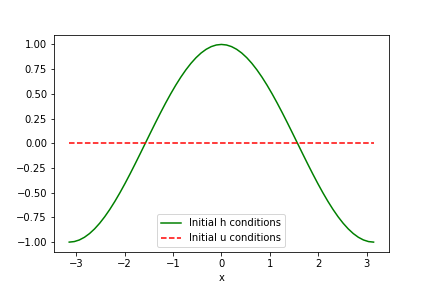
\includegraphics[width=\textwidth]{initial_condition_cos.png}
	\caption{\label{initialconditioncos}Initial conditions such that $u$ is zero everywhere and $h = \cos(x)$}
\end{minipage}
	\begin{minipage}{.5\textwidth}
	\ContinuedFloat
	%\centering
	\captionsetup{width=0.9\textwidth}
	\captionsetup{justification=centering}
	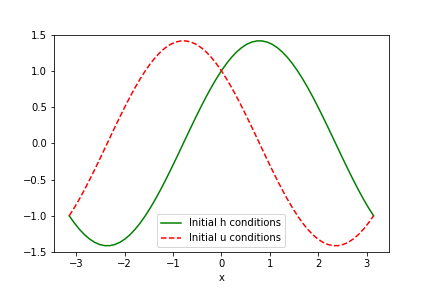
\includegraphics[width=\textwidth]{initial_condition_cossin.png}
	\caption{\label{initialconditioncossin}Initial conditions such that $u = \cos(x) - \sin(x)$ and $h = \cos(x) + \sin(x)$}
\end{minipage}
\end{figure}

First, we compare the results of our numerical methods with the analytic solution. We start with the initial conditions 
\begin{eqnarray}
u  & =  & 0 \\
h & = &  \cos(x)
\end{eqnarray}
shown in Figure \ref{initialconditioncos} for which it is possible to find an analytic solution of the shallow water equations:
\begin{equation}\label{uanalytic}
u = \sin(x)\sin(t)
\end{equation}
\begin{equation}\label{hanalytic}
h = \cos(x)\cos(t).
\end{equation}
These solutions are periodic, if $x$ is defined on the interval $[-\pi, \pi]$. Additionally we define  $c = 0.1$, $nx = 100$ and $nt = 100$.


\renewcommand\theContinuedFloat{\alph{ContinuedFloat}}
\begin{figure} [H]
	\begin{minipage}{.5\textwidth}
		\ContinuedFloat*
		%\centering
		\captionsetup{width=0.9\textwidth}
		\captionsetup{justification=centering}
		\includegraphics[width=\textwidth]{comparison_with_analytic_u.png}
		\caption{\label{exact velocity} Velocity, $u$, for the initial conditions shown in Figure \ref{initialconditioncossin}. } 
	\end{minipage}
	\begin{minipage}{.5\textwidth}
		\ContinuedFloat
		%\centering
		\captionsetup{width=0.9\textwidth}
		\captionsetup{justification=centering}
		\includegraphics[width=\textwidth]{comparison_with_analytic_h.png}
		\caption{\label{exact height} Height, $h$, for the initial conditions shown in Figure \ref{initialconditioncossin}.} 
	\end{minipage}
\end{figure}

Figures \ref{exact velocity} and \ref{exact height} show that all the numerical methods approximate very closely to the analytic solution for the smooth initial conditions $u= 0$ and $h= \cos(x)$. To see the error between the numerical method solution $u$ and the analytic solution $U$, we calculate the l2 error norms of the schemes, for example for $u$
\begin{equation}
\text{error in } u = \frac{\lvert \lvert u - U\rvert\rvert_{2}}{\lvert \lvert U\rvert\rvert _{2}} = \frac{\sqrt{\sum_{j} \lvert u_{j}^{n} - U(j\Delta x, n\Delta t\rvert^{2})}}{\sqrt{\sum_{j} \lvert U(j\Delta x, n\Delta t)\rvert^{2}}}
\end{equation}
These error norms are displayed in Table \ref{errortable} and show that the staggered semi-implicit method is the most accurate for both $u$ and $h$, as expected, because it is second order in time and space whereas the other schemes are only first order in time and second order in space. The co-located implicit scheme is slightly more inaccurate than the other schemes for $u$. This may be because of cumulative errors when inverting and multiplying the matrix used in the scheme.

\begin{table}[H]
	\centering
	\begin{tabular}{|c | c| c|} 
		\hline
		\textbf{Numerical Method} & \textbf{Error in u} & \textbf{Error in h}  \\
		\hline
		Co-located Explicit & $5.6 \times 10^{-4}$ & $2.0 \times 10^{-3}$\\ 
		\hline
		Staggered Explicit &  $1.5 \times 10^{-4}$ & $2.1 \times 10^{-3}$\\
		\hline
		Co-located  Implicit & $2.5 \times 10^{-3}$ & $1.7 \times 10^{-3}$ \\
		\hline
		Staggered Semi-implicit & $1.4 \times 10^{-4}$ & $7.7\times 10 ^{-5}$ \\
	\hline
	\end{tabular}
	\caption{l2 error norms for all 4 numerical methods}
	\label{errortable}
\end{table}

To test whether the numerical methods approximate the analytic solution for other initial conditions, we can take different initial conditions
\begin{eqnarray} \label{ic}
u  =  \cos(x) - \sin(x)\\
 h  =  \cos(x) + \sin(x)
\end{eqnarray}
(shown in Figure \ref{initialconditioncossin})for which we can also find an analytic solution of the shallow water equations:
\begin{eqnarray} \label{as}
u = (\cos(x) - \sin(x))(\cos(t) - \sin(t))\\
h = (\cos(x) + \sin(x))(\cos(t) + \sin(t))
\end{eqnarray}
Again we choose $x$ in the interval $[-\pi, \pi]$ so that these solutions are periodic. By using these initial conditions and analytic solution we can test whether the orders of accuracy with respect to $\Delta x$ and $\Delta t$ found by Taylor series expansion analysis in section \ref{numericalmethodssection} are correct, by using these initial conditions and analytic solution. For a fixed Courant number and fixed $x$ domain and total time, varying $\Delta x$, varies $\Delta t$ too which means that plotting the error against either $\Delta x$ or $\Delta t$ gives the same result.  

We use a large Courant number of $c = 0.5$ to find the order of the error with respect to $\Delta t$, as $c \propto \frac{\Delta t}{\Delta x}$, and so $\Delta t$ dominates for large Courant numbers. We find the error of the solution at time $\frac{\pi}{12}$ for $nx = [120, 240, 360, 480]$ and $nt = [10, 20, 30, 40]$ on the domain $-\pi \leq x \leq \pi$. The results of this test are displayed in Figures \ref{uerrorcossindt} and \ref{herrorcossindt}.

We repeat this process with a small Courant number of $c = 0.005$ to find the order of the error with respect to $\Delta x$, we repeat this process, as $c \propto \frac{\Delta t}{\Delta x}$ and so $\Delta x$ dominates for small Courant numbers. We find the error of the solution at time $\pi$ for $nx = [12, 24, 36, 48]$ and $nt = [1200, 2400, 3600, 4800]$ on the domain $-\pi \leq x \leq \pi$. The results of this test are displayed in Figures \ref{uerrorcossindx} and \ref{herrorcossindx}.

\begin{figure} [H]
	\begin{minipage}{.5\textwidth}
		\ContinuedFloat*
		%\centering
		\captionsetup{width=0.9\textwidth}
		\captionsetup{justification=centering}
		\includegraphics[width=\textwidth]{{uerror_compared_dt_cossin_c=0.5}.png}
		\caption{\label{uerrorcossindt}Log plot of l2 error norm of $u$ vs $\Delta t$ where $c = 0.1$. Lines proportional to $\Delta t$ and $\Delta t^{2}$ are plotted for reference.} 
	\end{minipage}
	\begin{minipage}{.5\textwidth}
		\ContinuedFloat
		%\centering
		\captionsetup{width=0.9\textwidth}
		\captionsetup{justification=centering}
		\includegraphics[width=\textwidth]{{herror_compared_dt_cossin_c=0.5}.png}
		\caption{\label{herrorcossindt}Log plot of l2 error norm of $h$ vs $\Delta t$ where $c= 0.1$. Lines proportional to $\Delta t$ and $\Delta t^{2}$ are plotted for reference.} 
	\end{minipage}
\end{figure}

\begin{figure}[H]
	\begin{minipage}{.5\textwidth}
		\ContinuedFloat*
		%\centering
		\captionsetup{width=0.9\textwidth}
		\captionsetup{justification=centering}
		\includegraphics[width=\textwidth]{{uerror_compared_dx_cossin_c=0.005}.png}
		\caption{\label{uerrorcossindx}Log plot of l2 error norm of $u$ vs $\Delta x$ where $c=0.005$. Lines proportional to $\Delta x^{2}$ are plotted for reference.} 
	\end{minipage}
	\begin{minipage}{.5\textwidth}
		\ContinuedFloat
		%\centering
		\captionsetup{width=0.9\textwidth}
		\captionsetup{justification=centering}
		\includegraphics[width=\textwidth]{{herror_compared_dx_cossin_c=0.005}.png}
		\caption{\label{herrorcossindx}Log plot of l2 error norm of $h$ vs $\Delta x$ where $c = 0.005$. Lines proportional to $\Delta x^{2}$ are plotted for reference.} 
	\end{minipage}
\end{figure}

The gradients of the lines plotted in Figures \ref{uerrorcossindt} - \ref{herrorcossindx}  are given in Tables \ref{gradientdt} and \ref{gradientdx}. These gradients are calculated using Python's least square polynomial fit function on the log relationships between the error and either $\Delta x$ or $\Delta t$ (choosing the polynomial to be order one). 

Our results agree closely with the order of accuracy calculated by the Taylor series expansion apart from for the time order of accuracy in the staggered explicit case. The reason may be that the scheme is already exhibiting instabilities (as it becomes unstable at $c = 1$.)


\begin{table}[H]
	\centering
	\begin{tabular}{|c | c| c| c|} 
		\hline
		\textbf{Numerical Method}  & $u$ error vs $\Delta t$ & $h$ error vs $\Delta t$ & Order in time \\
		\hline
		Co-located Explicit & 1.02 & 1.01 & 1\\ 
		\hline
		Staggered Explicit & 0.13 & 0.02 & 1\\
		\hline
		Co-located Implicit & 0.95 & 1.01 & 1\\
		\hline
		Staggered Implicit & 2.00 & 2.00 & 2\\
		\hline
	\end{tabular}
	\caption{Time order of accuracy from numerical methods taken from Figures \ref{uerrorcossindt} - \ref{herrorcossindt} compared to spatial order of accuracy from Taylor series expansion}
	\label{gradientdt}
\end{table}

\begin{table}[H]
	\centering
	\begin{tabular}{|c | c| c| c|} 
		\hline
		\textbf{Numerical Method} & $u$ error vs $\Delta x$ &  $h$ error vs $\Delta x$ & Order in space\\
		\hline
		Co-located Explicit & 1.94 & 2.03 & 2 \\ 
		\hline
		Staggered Explicit & 1.93 & 1.99 & 2 \\
		\hline
		Co-located Implicit & 2.00 & 1.97 & 2 \\
		\hline
		Staggered Implicit & 1.99 & 2.01 & 2 \\
		\hline
	\end{tabular}
	\caption{Spatial order of accuracy from numerical methods taken from Figures \ref{uerrorcossindx} - \ref{herrorcossindx} compared to spatial order of accuracy from Taylor series expansion}
	\label{gradientdx}
\end{table}

Next we test some of the numerical properties of the schemes.
\subsection{Test 1}
Using Von-Neumann stability analysis above, we found that the co-located explicit scheme is unstable for Courant numbers higher than 2, but that the co-located implicit scheme is unconditionally stable (\textit{ie.} stable for all Courant numbers). To test this result, we run both schemes using a range of Courant numbers with the initial conditions $h = \cos(x) + \sin(x)$ and $u = \cos(x) -\sin(x)$ (shown in Figure \ref{initialconditioncossin}), plus $nx = 100$ and $nt = 100$.

For Courant numbers larger than $2$, Figures \ref{velocity_varying_courant} and \ref{height_varying_courant} show that the co-located explicit scheme is unstable for both $u$ and $h$. By contrast, for large Courant numbers, the co-located implicit scheme remains stable for $u$ and $h$. This is as expected from the Von-Neumann stability analysis.

\begin{figure}[H]
	\begin{minipage}{.5\textwidth}
		\ContinuedFloat*
		%\centering
		\captionsetup{width=0.9\textwidth}
		\captionsetup{justification=centering}
		\includegraphics[width=\textwidth]{velocity_varying_courant.png}
		\caption{\label{velocity_varying_courant} Velocity for varying Courant numbers for the co-located explicit and implicit schemes} 
	\end{minipage}
	\begin{minipage}{.5\textwidth}
	\ContinuedFloat
	%\centering
	\captionsetup{width=0.9\textwidth}
	\captionsetup{justification=centering}
	\includegraphics[width=\textwidth]{height_varying_courant.png}
	\caption{\label{height_varying_courant} Height for varying Courant numbers for the co-located explicit and implicit methods} 
\end{minipage}
\end{figure}

\subsection{Test 2}
\begin{figure}[H]
\begin{center}
\begin{minipage}{.5\textwidth}
	\centering
	\captionsetup{width=2\textwidth}
	\captionsetup{justification=centering}
	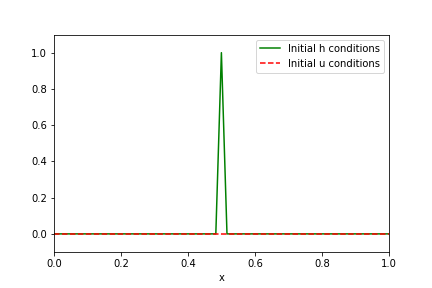
\includegraphics[width=\textwidth]{initial_condition_spike.png}
	\caption{\label{initialconditionspike}Initial conditions such that $u$ and $h$ are zero everywhere apart from one point at the centre where $h = 1$} 
\end{minipage}
\end{center}
\end{figure}

When looking at the dispersion relation for the co-located grid scheme above, it seemed that the results produced may be unphysical, as the wave produced by the numerical scheme propagates much more slowly than the analytic solution and the wave frequency does not increase as $k\Delta x$ increases. By contrast, we expect the staggered grid to produce more physical results. We test this hypothesis by taking the different and less smooth initial conditions that both $u$ and $h$ are zero everywhere apart from one point in the centre where $h = 1$ (as shown in Figure \ref{initialconditionspike}). We then plot the solutions of $u$ and $h$ at multiple time steps for the co-located explicit scheme and the staggered explicit scheme in Figures \ref{velocity_spike} and \ref{height_spike}.

For this test we use $nx = 20$ and $nt = 10$ on the $x$ domain $0 \leq x \leq 1$ and a Courant number of $0.1$.

\begin{figure} [H]
	\begin{center}
	\begin{minipage}{.6\textwidth}
		\ContinuedFloat*
		%\centering
		\captionsetup{width=1.5\textwidth}
		\captionsetup{justification=centering}
		\includegraphics[width=\textwidth]{velocity_spike.png}
		\caption{\label{velocity_spike} Velocity at different timesteps using the co-located explicit scheme and the staggered explicit scheme} 
	\end{minipage}
\end{center}
\end{figure}
\begin{figure}[H]
	\begin{center}
	\begin{minipage}{.6\textwidth}
		\ContinuedFloat
		%\centering
		\captionsetup{width=1.5\textwidth}
		\captionsetup{justification=centering}
		\includegraphics[width=\textwidth]{height_spike.png}
		\caption{\label{height_spike} Height at different timesteps using the co-located explicit scheme and the staggered explicit scheme} 
	\end{minipage}
\end{center}
\end{figure}

As expected the results shown in Figures \ref{velocity_spike} and \ref{height_spike} for the co-located grid are unphysical. The fluid does spread out but it does not go to the next meshpoint. Instead, it skips this meshpoint out and moves to the next meshpoint along. In Figure \ref{height_spike} we see that the two points around the central grid point ($x_{m}$ hereafter) never have any height for the co-located grid. This means that the fluid passes from $x_{m}$ to $x_{m-2}$ and $x_{m+ 2}$ without passing through $x_{m-1}$ and $x_{m+1}$ which is clearly unphysical. Similarly, for the co-located grid in Figure \ref{velocity_spike} there is never any velocity at the gridpoints $x_{m-2}$ and $x_{m+2}$ for the co-located grid which is also unphysical. 

In contrast, the staggered scheme produces physically realistic results for these initial conditions. Figure \ref{velocity_spike} shows that the velocity is non-zero at the gridpoints where the wave has propagated as expected from a physical system and Figure \ref{height_spike} shows that the height spreads out evenly using all grid points.


\subsection{Test 3}
Finally, we compare the computational cost of the four numerical methods by comparing the time it takes for each of them to run for each initial condition: $u$ is zero everywhere and $h= \cos(x)$ shown in Figure \ref{initialconditioncos}; $u = \cos(x) - \sin(x)$ and $h = \cos(x) + \sin(x)$ shown in Figure \ref{initialconditioncossin} and $u$ and $h$ are zero everywhere apart from one point in the centre where $h = $. The scheme have been run on an $x$-domain of $-\pi \leq x \leq \pi$, with Courant number $0.1$ and with the same number of time steps ($nt = 1000$) and space steps ($nx = 1000$).

\begin{table}[H]
	\centering
	\begin{tabular}{|c | c| c| c|} 
		\hline
		\textbf{Numerical Method} & \textbf{Time IC Fig \ref{initialconditioncos}} &  \textbf{Time IC Fig \ref{initialconditioncossin}}  & \textbf{Time IC Fig \ref{initialconditionspike}} \\
		\hline
		Co-located Explicit & 1.76 s & 1.77 s & 1.82 s\\ 
		\hline
		Staggered Explicit & 1.58 s &1.58 s & 1.59 s\\
		\hline
		Co-located  Implicit & 3.05 s &3.05 s & 2.97 s\\
		\hline
		Staggered Implicit & 5.21 s &5.27 s & 5.16 s\\
		\hline
	\end{tabular}
	\caption{Time taken (3sf) for each numerical method to run for every set of initial conditions.}
	\label{timingtable}
\end{table}

As we would expect there is very little difference between the time each scheme takes to run for each initial condition. This is as expected as the time should be dependent on the computational cost of the scheme.

Furthermore, as expected, the co-located explicit and staggered explicit methods take a similar amount of time because they have the same number of floating point operations per iteration. 

The implicit methods have a higher computational cost and take longer than the explicit methods as expected. This is because they involve one inversion of a matrix (O($n^{3}$) floating point operations for an $n \times n$ matrix) and a matrix-vector multiplication (O($n^{2}$) floating point operations for an $n \times n$ matrix) at each iteration to find $u^{m}$ or $h^{m}$.

The staggered implicit method has the highest computational cost and takes the longest time because constructing $b_{i}$ in the $A_{ij}x_{j} = b_{i}$ matrix equation involves nine floating point operations compared to three to construct $b_{i}$ in the co-located implicit method. Therefore it takes the longest of the four numerical methods.  

\section{Conclusions}

From the results listed in Section \ref{resultssection}, we can conclude the following:

\begin{itemize}
	\item The implicit staggered method is the most accurate of the four numerical methods;
	\item When working with high Courant numbers (e.g. when the meshgrid spacing is very fine so $\Delta x$ is small or when $H$ or $\Delta t$ are very large), it is better to choose implicit methods because they are stable for all Courant numbers, unlike the explicit methods (see Test 1);
	\item Staggered grids produce more physically realistic results than co-located grids for certain initial conditions (see Test 2);
	\item When working with small Courant numbers, it is better to choose explicit methods because they are less computationally expensive than implicit methods (see Test 3).
\end{itemize}


\begin{thebibliography}{9}
	\addcontentsline{toc}{part}{Bibliography}
	\bibitem{MPE textbook}
	Cotter, C. and Weller, H., (2018), \textquoteleft Numerical Methods\textquoteright, Ch.5 in Crisan, D (ed.), \textit{Mathematics of Planet Earth: A primer}, World Scientific Publishing Europe Ltd., London.
	\bibitem{implicit}
	Casulli, V. and Cattani, E., (1994), \textquoteleft Stability, Accuracy and Efficiency of a Semi-Implicit Method for Three-Dimensional Shallow Water Flow\textquoteright, \textit{Computers Math. Applic}, \textbf{27(4)}, 99-112.
\end{thebibliography}
\end{document}